\section{Deliberative Reasoning and Planning}

\begin{frame}{}
    \LARGE Advanced Reasoning: \textbf{Deliberative Reasoning and Planning}

    \vspace{1em}
    \normalsize Reasoning models are called ``System 2''. Can they plan, and are their traces really deliberation?
\end{frame}

\begin{frame}{PlanBench: From ``Cannot Plan'' to Saturated in Two Years}
    \begin{columns}[T,onlytextwidth]
        \column{0.5\textwidth}
        \centering
        \begin{adjustbox}{max width=\linewidth}\begin{tikzpicture}
            \begin{axis}[ybar, width=7.4cm, height=5.6cm, bar width=0.26cm,
                ymin=0, ymax=118, ylabel={\scriptsize plans correct (\%)},
                symbolic x coords={Classic, Mystery, Randomised}, xtick=data,
                x tick label style={font=\scriptsize}, y tick label style={font=\scriptsize},
                nodes near coords, nodes near coords style={font=\tiny, rotate=90, anchor=west},
                legend style={font=\tiny, at={(0.5,1.02)}, anchor=south, legend columns=4, draw=none},
                axis lines=left, enlarge x limits=0.25]
                \addplot[fill=gray!35, draw=gray] coordinates {(Classic,35.5) (Mystery,0) (Randomised,0.83)};
                \addplot[fill=KAUSTcyan!30, draw=KAUSTcyan!70!black] coordinates {(Classic,56.7) (Mystery,19.1) (Randomised,9.33)};
                \addplot[fill=KAUSTcyan!70, draw=KAUSTcyan!70!black] coordinates {(Classic,95.7) (Mystery,74.3) (Randomised,31.5)};
                \addplot[fill=darkorange!60, draw=darkorange!80!black] coordinates {(Classic,99.3) (Mystery,98.1) (Randomised,92.5)};
                \addlegendentry{GPT-4o}
                \addlegendentry{o1-mini}
                \addlegendentry{o1}
                \addlegendentry{GPT-5}
            \end{axis}
        \end{tikzpicture}\end{adjustbox}

        {\scriptsize Blocksworld with plain prompts. Mystery and Randomised hide the names.}
        \column{0.48\textwidth}
        \begin{itemize}\itemsep0.45em
            \item \textbf{PlanBench} separates planning from recall. \emph{Mystery} Blocksworld obfuscates the names, so memorised patterns stop working.
            \item \textbf{2024:} the best plain LLM reaches 62.6\% on Blocksworld. None passes 5\% on Mystery.
            \item \textbf{o1-preview:} 97.8\% and 52.8\%, at \$42 per 100 instances and 40 to 111 seconds each. The classical planner Fast Downward: 100\% in 0.12 seconds.
            \item \textbf{GPT-5:} the obfuscated variants are close to solved.
        \end{itemize}
    \end{columns}
    \vspace{0.1em}
    \src{Chart: Goh, Kos and Goel, ``Knowledge Model Prompting Increases LLM Performance on Planning Tasks,'' \href{https://arxiv.org/abs/2602.03900}{arXiv:2602.03900}, Table 2. Valmeekam et al., ``PlanBench,'' \href{https://arxiv.org/abs/2206.10498}{arXiv:2206.10498}, and ``Planning in Strawberry Fields,'' \href{https://arxiv.org/abs/2410.02162}{arXiv:2410.02162}.}
\end{frame}

\begin{frame}{What Is Not Solved: Long Plans and Impossible Problems}
    \begin{columns}[T,onlytextwidth]
        \column{0.5\textwidth}
        \centering
        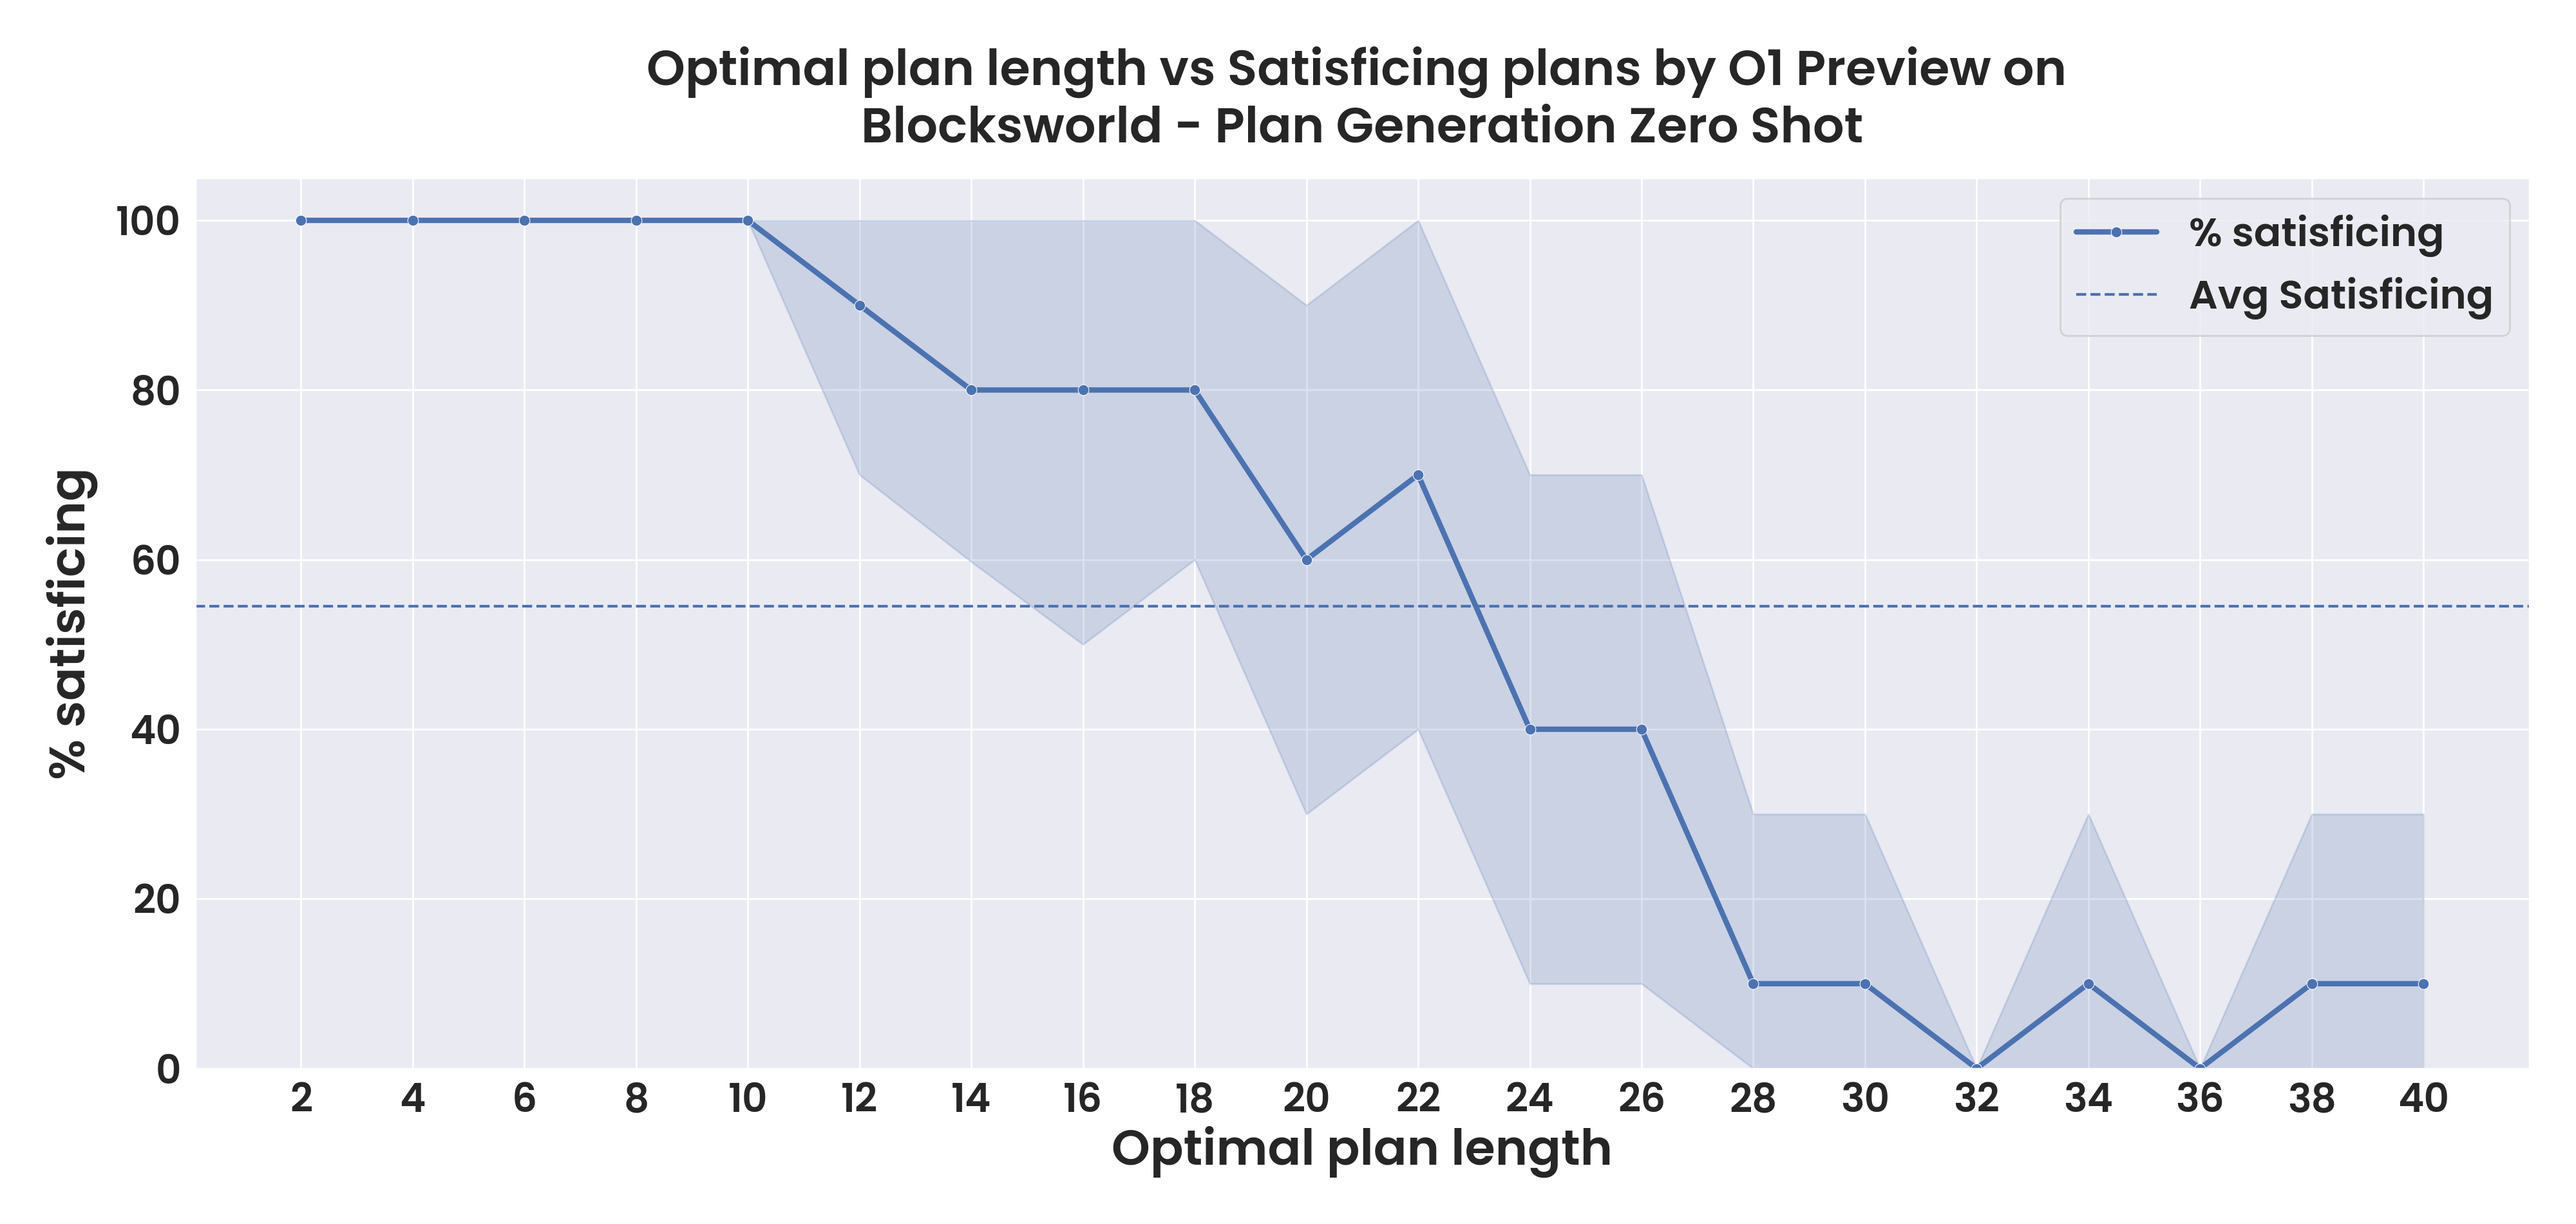
\includegraphics[width=\linewidth,height=0.42\textheight,keepaspectratio]{images/advanced-reasoning/strawberry_plan_length.png}

        {\scriptsize o1-preview on Blocksworld, by length of the optimal plan}
        \column{0.48\textwidth}
        \begin{itemize}\itemsep0.45em
            \item \textbf{Horizon.} On plans of 20 to 40 steps, o1-preview falls to 23.6\%.
            \item \textbf{Unsolvable instances.} It recognises only 27\% of them, and declares 11.5\% of solvable problems impossible.
            \item \textbf{Agentic planning (2026).} PlanBench-XL: 327 retail tasks over 1,665 tools. GPT-5.4 scores 51.9\%, and \alert{11.4\%} when tools fail or vanish without a clear error.
        \end{itemize}
    \end{columns}
    \vspace{0.2em}
    \caveat{No newer public numbers were found for long horizons or unsolvability. ``Blocksworld is saturated'' is not ``planning is solved''.}
    \src{Valmeekam et al., \href{https://arxiv.org/abs/2409.13373}{arXiv:2409.13373}, and ``Planning in Strawberry Fields,'' \href{https://arxiv.org/abs/2410.02162}{arXiv:2410.02162}. Liu et al., ``PlanBench-XL,'' \href{https://arxiv.org/abs/2606.22388}{arXiv:2606.22388}.}
\end{frame}

\begin{frame}{LLM-Modulo: Put a Sound Verifier in the Loop}
    \begin{columns}[T,onlytextwidth]
        \column{0.5\textwidth}
        \centering
        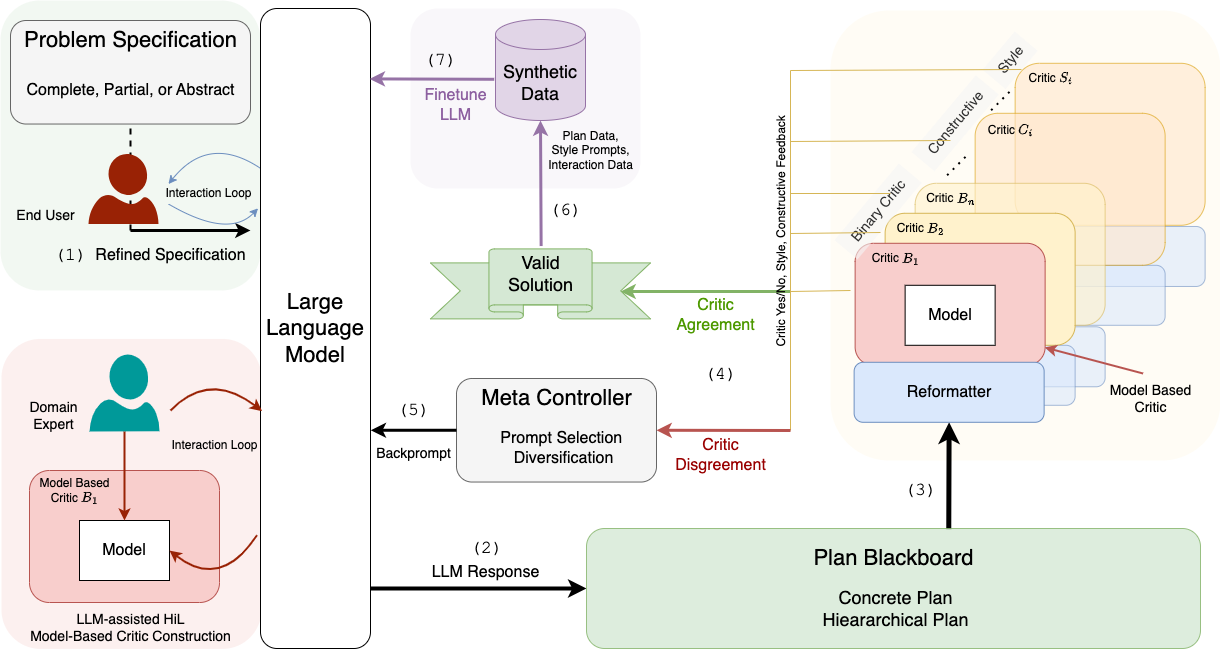
\includegraphics[width=\linewidth,height=0.6\textheight,keepaspectratio]{images/advanced-reasoning/llm_modulo_fig3_framework.png}
        \column{0.48\textwidth}
        \begin{itemize}\itemsep0.45em
            \item \textbf{Position:} LLMs cannot plan or verify alone, but they are good \emph{generators} of candidates.
            \item \textbf{Architecture:} generate, test, critique.
            \begin{itemize}\itemsep0.1em
                \item \emph{hard} critics are model-based and sound
                \item \emph{soft} critics judge style
                \item a meta-controller turns the critiques into the next prompt
            \end{itemize}
            \item GPT-4 alone: about 12\% of plans executable. With verifier feedback: 82\% on Blocksworld within 15 rounds.
            \item \textbf{LLM+P} is the other design: the LLM only \emph{translates} the problem into PDDL, and a classical planner solves it. Blocksworld: 20\% to 90\%.
        \end{itemize}
    \end{columns}
    \vspace{0.1em}
    \src{Kambhampati et al., ``LLMs Can't Plan, But Can Help Planning in LLM-Modulo Frameworks,'' ICML 2024, \href{https://arxiv.org/abs/2402.01817}{arXiv:2402.01817}, Figure 3. Liu et al., ``LLM+P,'' \href{https://arxiv.org/abs/2304.11477}{arXiv:2304.11477}, Table I.}
\end{frame}

\begin{frame}{The Same Loop with a Reasoning Model, and Then Inside Training}
    \begin{center}
    \small
    \begin{adjustbox}{max width=\linewidth}\begin{tabular}{llccc}
        \toprule
        \textbf{Task} & \textbf{Model} & \textbf{Direct} & \textbf{With verifier loop} & \textbf{Rounds} \\
        \midrule
        \rowcolor{KAUSTcyan!12} Blocksworld, 20 or more steps & o1-preview & 23.65\% & \textbf{98.2\%} & 7 \\
        Blocksworld, 20 or more steps & o1-mini & 0.90\% & 10\% & 4 \\
        Hard graph colouring & o1-preview & & 94\% & 10 \\
        TravelPlanner & o1-preview & & 65\% & 10 \\
        \bottomrule
    \end{tabular}\end{adjustbox}
    \end{center}
    \begin{itemize}\itemsep0.4em
        \item A sound verifier turns a 24\% planner into a 98\% one. It does not rescue a weak generator.
        \item \textbf{2026: the verifier's signal moves into training.}
        \begin{itemize}\itemsep0.15em
            \item \emph{Solver-feedback RL.} A 7B model learns to write PDDL from solver feedback alone, in three roles: actor, judge, editor. Average success 70.8\% against 35.5\% for LLM+P.
            \item It also drifts less from the intended meaning: 6.4\% against 20.4\%.
            \item \emph{HALO.} A small trained orchestrator matches an API-model orchestrator at \$0.004 per task instead of \$0.18.
        \end{itemize}
    \end{itemize}
    \src{Valmeekam et al., ``Planning in Strawberry Fields,'' \href{https://arxiv.org/abs/2410.02162}{arXiv:2410.02162}. Zhang et al., ``From Solver Feedback to Faithful Plans,'' \href{https://arxiv.org/abs/2608.21897}{arXiv:2608.21897}, Tables 1 and 3. Mangannavar et al. (HALO), \href{https://arxiv.org/abs/2606.21740}{arXiv:2606.21740} (abstract).}
\end{frame}

\begin{frame}{Are the Traces Deliberation?}
    \begin{itemize}\itemsep0.6em
        \item The popular frame: base LLMs are ``System 1'', reasoning models ``System 2''.
        \item \textbf{The counter-position:} intermediate tokens are \emph{learned prompt augmentations}, not interpretable reasoning.
        \item \textbf{Evidence:} transformers trained on \emph{corrupted} search traces do about as well as those trained on correct ones. GRPO raises answer accuracy without raising trace validity.
        \item The other side sees a real, learned search. That is the next section.
    \end{itemize}
    \vspace{0.4em}
    \takeaway{A trace that improves the answer need not be a faithful record of how the answer was found.}
    \src{Li et al., ``From System 1 to System 2,'' \href{https://arxiv.org/abs/2502.17419}{arXiv:2502.17419}. Kambhampati et al., ``Stop Anthropomorphizing Intermediate Tokens as Reasoning/Thinking Traces!'' ICML 2026, \href{https://arxiv.org/abs/2504.09762}{arXiv:2504.09762}. Valmeekam et al., ``Beyond Semantics,'' \href{https://arxiv.org/abs/2505.13775}{arXiv:2505.13775}.}
\end{frame}

\begin{frame}{Planning: What to Remember}
    \begin{itemize}\itemsep0.6em
        \item Reasoning models moved classical planning benchmarks from \textbf{under 5\% to above 90\%} on obfuscated Blocksworld.
        \item What remains open: \textbf{long horizons, unsolvable instances, tool failures}, and cost against a classical planner.
        \item A \textbf{sound verifier in the loop} gives guarantees the model cannot. In 2026 its signal is used for training too.
        \item Whether traces are ``reasoning'' is unsettled. Their usefulness does not depend on the answer.
    \end{itemize}
    \vspace{0.3em}
    \vspace{0.3em}
    \takeaway{\textbf{Next.} So far, search and verification sat outside the model. Can the search itself be written into the tokens, and learned?}
\end{frame}
